\chapter{Ranking-Based Semantics} \label{Ranking-Based Semantics}
\section{Scelta dell’argomento migliore}
Un ranking è un ordinamento parziale o totale di un insieme di argomenti. Quello che ottengo da una semantica di ranking è un vero e proprio ordinamento, cioè una cosa del tipo:
\begin{center}
    $a > d > c > e >b$
\end{center}
e non un insieme come lo era fino ad adesso. Quindi potremo dire quando un argomento è ”migliore” rispetto ad un altro. Possiamo avere:
\begin{itemize}
    \item Ordinamento \textbf{quantitativo:} Consiste nell’assegnare prima dei punteggi agli argomenti come "a vale 5, b vale 7" quindi concludo che b è migliore.
    \item Ordinamento \textbf{qualitativo}: "Seguendo questo ordinamento l’argomento a è migliore dell’argomento d.
\end{itemize}
\begin{center}
    Metodi visti
\end{center}
\begin{enumerate}
    \item Categorizer
    \item Graded Defense: $a_1 \in d^1_{1} (X_1)$
    \item Shapley Value
\end{enumerate}
\section{Ordinamento quantitativo}
\subsection{Categorizer}
Ordina gli argomenti utilizzando la seguente funzione:
\begin{enumerate}
    \item Per ogni argomento guarda il numero degli attacchi che riceve.
    \item Utilizza questo valore per assegnare un ranking a tale argomento.
\end{enumerate}
\textbf{In altre parole abbiamo:} Se sono attaccato da argomenti deboli allora sono un argomento forte; se sono attaccato da argomenti forti sono un argomento debole.
\begin{figure}[htp]
	\centering
    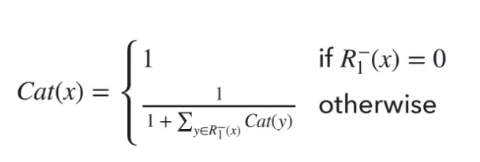
\includegraphics[width=10cm, keepaspectratio]{img/Cap8/quantitativo1.png}
    \caption{Funzione categorizer.}
\end{figure}
Se un argomento non ha attaccanti $R^-1$ $(x) = 0$ allora il valore è 1 sennò è dato 1 dalla formula
$\frac{1}{1+\sum_{y\in R^-1_(x)} Cat(y)}$, questo significa che se ho attaccanti forti allora l’argomento x è debole
\newpage
\begin{figure}[htp]
	\centering
    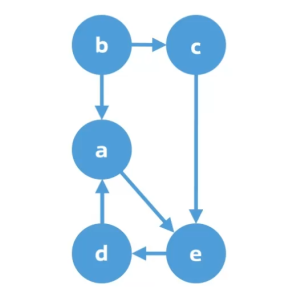
\includegraphics[width=10cm, keepaspectratio]{img/Cap8/quantitativo2.png}
    \caption{Esempio categorizer.}
\end{figure}
\textbf{Spiegazione: } Si parte sempre dagli iniziatori del grafo, cioè gli argomenti non attaccati.
\begin{itemize}
    \item $b:$ Ha valore 1 perchè la frase: ”non ha attaccanti” si traduce in $R^-_1(x) = 0$ quindi va nella prima opzione della funzione, si arresta subito e torna 1.
    \item $c:$ Non vale la prima opzione perchè è attaccato da b, quindi seconda opzione e calcolo 1 + la sommatoria dei valori dei suoi attaccanti cioè 1 solamente b. Quindi verrebbe $\frac{1}{1+1}$ = 0.5
\end{itemize}
In questo caso Cat(b)=1 perchè non ha attaccanti e Cat(c)=0.5 perchè è attaccato da b con punteggio 1. Mentre Cat(a)=0.38, Cat(d) =0.65 e Cat(e) = 0.53.

\vspace{0.3cm}

Si continua cosi per tutti gli argomenti. Infine si ordinano i risultati e si ottiene un ordinamento sui rispettivi argomenti:
\begin{center}
    $b>d>e>c>a$
\end{center}
Quindi $b$ è preferito tramite la funzione $cat$ a $d$ e cosi via.
\section{Ordinamento Qualitativo}
I principi sono simili a quello precedente:
\begin{itemize}
    \item più è grande il numero degli attaccanti su un argomento b, più è debole il livello di giustificazione di b
    \item più è grande il numero di argomenti che difendono a, più è forte il livello di giustificazione di a.
\end{itemize}
\subsection{Graded Defense, Dung’s Theory}
In questo caso andiamo a definire una relazione di preferenza tra le coppie dei possibili argomenti \textbf{(non si assegnano punteggi)}. I principi che utilizzeremo sono due:
\begin{enumerate}
    \item Più attaccanti un argomento ha, peggiore è quell’argomento.
    \item Più argomenti sono in mia difesa, più un argomento è forte.
    
\end{enumerate}
Suddivido gli argomenti con la \textbf{funzione}: $d^m_n$ (X) che rappresenta tutti quegli argomenti che \textbf{non} hanno almeno $m$ attaccanti che a loro volta \textbf{non} sono contrattaccati da almeno $n$ argomenti.

\vspace{0.3cm}

\textbf{Esempio}

\begin{figure}[htp]
	\centering
    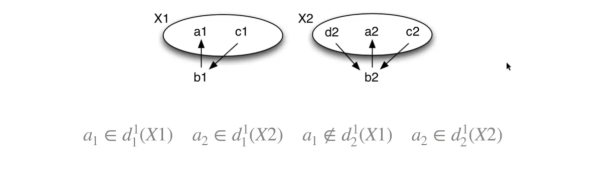
\includegraphics[width=13cm, keepaspectratio]{img/Cap8/defense.png}
    \caption{Esempio graded defense.}
\end{figure}
$a_1$ ha un attaccante ed un difensore, quindi appartiene. a1 ha si un attaccante, ma non ha due difensori, quindi non appartiene.
\newpage
\begin{itemize}
    \item $a_1 \in d^1_1$ (X1): non c’è almeno 1 attaccante che non sia attaccato a sua volta da almeno 1 argomento. Questo vuol dire che c’è almeno un argomento che è contrattaccato da almeno un altro argomento. Infatti a1 è attaccato da b1 che è a sua volta attaccato da c1 .
    \item $a_2 \in d^1_1$ (X2): non c’è un argomento che attacca a2 che a sua volta non sia contrattaccato da almeno un altro argomento, ma addirittura $c_i$ sono due argomenti (che sarebbero $d_2$ , $c_2$ ) che contrattaccano l’attaccante di $a_2$ (che sarebbe $b_2$ ), quindi diciamo anche che $a_2 \in d^2_1$ (X2). (Esiste un attaccante di $a_1$ ma non esistono due difensori di $a_1$).
\end{itemize}
\begin{center}
    $a_2 \in d^1_2$ (X2)
\end{center}
Va letto come: Non esiste un argomento (quindi prima l’esponente) che non sia contrattaccato da almeno 2 argomenti (quindi poi il pedice). Gli attaccanti li leggo ad apice, i difensori (cioè chi attacca il mio attaccante) li leggo a pedice. Il dilemma che ci troviamo davanti è:
\begin{center}
    É meglio essere poco attaccati (cioè apice basso) o è meglio avere tanti difensori (pedice alto?)
\end{center}
In formule sarebbe: appartenere a $d^3_1$ è meglio o peggio di appartenere a $d^1_3?$
\subsection{Formula}
\begin{center}
    $d^m_n$ è meglio di $d^s_t$ $\Leftarrow \Rightarrow$ m $<=$ s AND t $<=$ n
\end{center}
Cioè un argomento non attaccato da almeno m argomenti che non siano contrattaccati da almeno n difensori è meglio della stessa cosa con s e t se e solo se il primo argomento ha sia \textbf{meno attaccanti}, cioè m $<=$ s che \textbf{più difensori} t $<=$ n.
\\Altri esempi: leggere solamente l’appartenenza
\begin{figure}[htp]
	\centering
    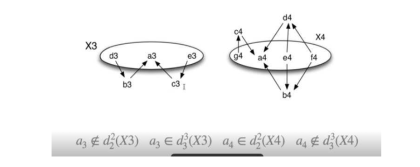
\includegraphics[width=13cm, keepaspectratio]{img/Cap8/defense2.png}
\end{figure}
\subsection{Applicazione della Graded Semantics ad un grafo}
\begin{figure}[htp]
	\centering
    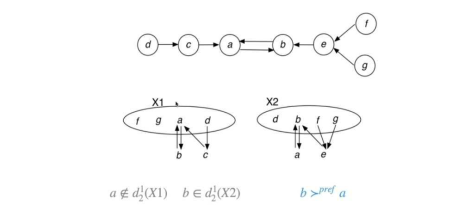
\includegraphics[width=13cm, keepaspectratio]{img/Cap8/GdefnseGrafo.png}
\end{figure}
\textbf{Ci domandiamo:} è vero che a $\in$ $d^1_2$ (X1)? 
\\Cioè è vero che a non è attaccato da almeno un argomento che non sia a sua volta attaccato da almeno due argomenti? 
\\NO, perchè a è attaccato da almeno 1 argomento, vero, ma questo argomento è attaccato da un solo argomento, che sarebbe d per c e a stesso per b. Il controllo sarebbe risultato vero che entrambi gli attaccanti venivano contrattaccati da almeno 2 argomenti.

\vspace{0.4cm}

\textbf{Ci domandiamo:} è vero che b $\in$ $d^1_2$ (X2)?, cioè è vero che b non è attaccato da un singolo argomento che a sua volta non sia contrattaccato da almeno due argomenti?
\begin{center}
    \textbf{Importante}
\end{center}
Si, perchè b è attaccato da almeno un argomento (e) che è a sua volta attaccato da almeno 2 argomenti, f e g.

\vspace{0.3cm}

Si vede per prima l’apice, e la domanda è: \textbf{quell’argomento è attaccato da almeno il numero che c’è scritto?}

\vspace{0.3cm}

Se la risposta è no allora sicuramente non appartiene, altrimenti si vede il numero in basso, cioè i difensori. 

\newpage
Se ad apice c’era 1 e a pedice 2 ci \textbf{chiediamo}:

\vspace{0.3cm}

C’è almeno 1 argomento che attacca a che è attaccato a sua volta da 2 argomenti? Se la risposta è si allora appartiene, no altrimenti.

\vspace{0.3cm}

Ora, la regola diceva che devo avere un minor numero di attaccanti e un maggior numero di difensori per essere un argomento migliore, quindi a ha lo stesso numero di attaccanti di b che sarebbe 2, il numero di difensori invece è pari a massimo 1 per a, mentre per b troviamo un contrattacco di 2
argomenti, quindi proprio perchè b ha più difensori di a, lo preferisco. quindi:
\begin{center}
    $b >^{pref}$ $a$
\end{center}
\section{Ordinamento Quantitativo: Shapley Value}
Negli AF va interpretato come "il valore che un argomento apporta dentro una certa estenzione".
\subsection{Assegnamento dei valori agli argomenti}
Devo calcolare lo Shapley value per ogni argomento data una certa semantica.
\\
Si utilizzano due funzioni, per gli IN e per gli OUT:
\begin{figure}[htp]
	\centering
    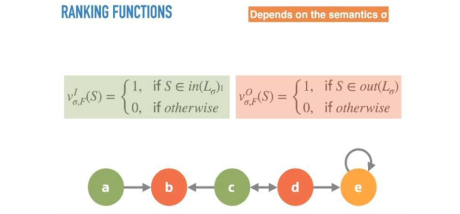
\includegraphics[width=13cm, keepaspectratio]{img/Cap8/ordinamento-quantitativo.png}
\end{figure}
\newpage
\begin{itemize}
    \item La funzione verde assegna agli argomenti il valore 1 se sono argomenti IN che sono accettati da qualche semantica $\sigma$, oppure 0. Se calcolo il valore per l’insieme a, c questo darà 1 perchè l’insieme è IN.
    \item La funzione rossa invece di guardare gli argomenti che sono IN e dargli punteggio 1, guarda quelli OUT e gli da punteggio 1 in maniera negativa.
\end{itemize}
Quindi se la funzione $V^I$ da punteggio 1 significa che sono una buona estensione, se la funzione $V^O$ da punteggio 1 allora sono una cattiva estensione. Adesso quindi siamo arrivati al punto di avere per ogni insieme di argomenti un valore che è 0 o 1 in base alla funzione per gli IN o per gli OUT e quindi possiamo generare un ordinamento.
\subsection{Ordinamento degli argomenti in base al valore}
\begin{figure}[htp]
	\centering
    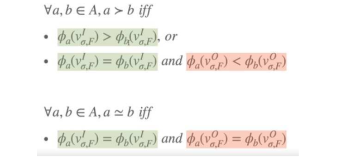
\includegraphics[width=10cm, keepaspectratio]{img/Cap8/ordinamento-valore.png}
\end{figure}
\textbf{Il primo punto si traduce in:}
\\L’argomento a è \textbf{migliore} dell’ argomento b se e soltanto se:
\begin{itemize}
    \item Lo shapley value di a rispetto agli argomenti IN è maggiore dello shapley value di b sempre rispetto agli argomenti IN.
    \item Oppure se il valore è uguale (quindi non mi basta andare a controllare solamente gli IN), a deve avere anche uno shapley value per gli OUT minore di quello di b.
\end{itemize}
\begin{center}
     \textbf{Il secondo punto è l’indifferenza}
\end{center}
 Scegliere prima a o b è indifferente se e soltanto se:
\begin{itemize}
    \item Lo shapley value per gli IN di a è esattamente uguale allo shapley value per gli IN di b e stessa cosa per il valore di OUT. 
\end{itemize}
    
    
